\section{Disorder Terms}


\begin{slide}{Structural Disorder and the Pair Distribution Function}

  \begin{cenpage}{135mm}

  An EXAFS measurement averages billions of {\BlueEmph{snapshots}} of the
  local structure:

\begin{cenpage}{88mm}
\begin{itemize}
\item Each absorbed x-ray generates 1 photo-electron.
\item the photo-electron / core-hole pair lives for about
  $10^{-15}$ s --  much faster than the thermal vibrations ($10^{-12}$ s).
\item An EXAFS measurement samples $10^4$ (dilute fluorescence) to $10^{10}$
  absorbed x-rays for each energy point.
\end{itemize}
\end{cenpage}

\vmm
 \vmm

So far, we've put this in the EXAFS Equation as \hspace{2mm}
$\chi \sim N \exp({-2k^2\sigma^2}) $

\vmm \hrule \vmm \onslide+<2->

\begin{columns}
  \begin{column}{70mm}
    More generally, EXAFS samples the

    \vmm
    {\RedEmph{Partial Pair Distribution Function}}

    \vmm

    {\RedEmph{$g(R)$}} =   probability that an
    atom is a distance $R$ away from the absorber.

    \vspace{8mm}

    \end{column}
  \begin{column}{65mm}

    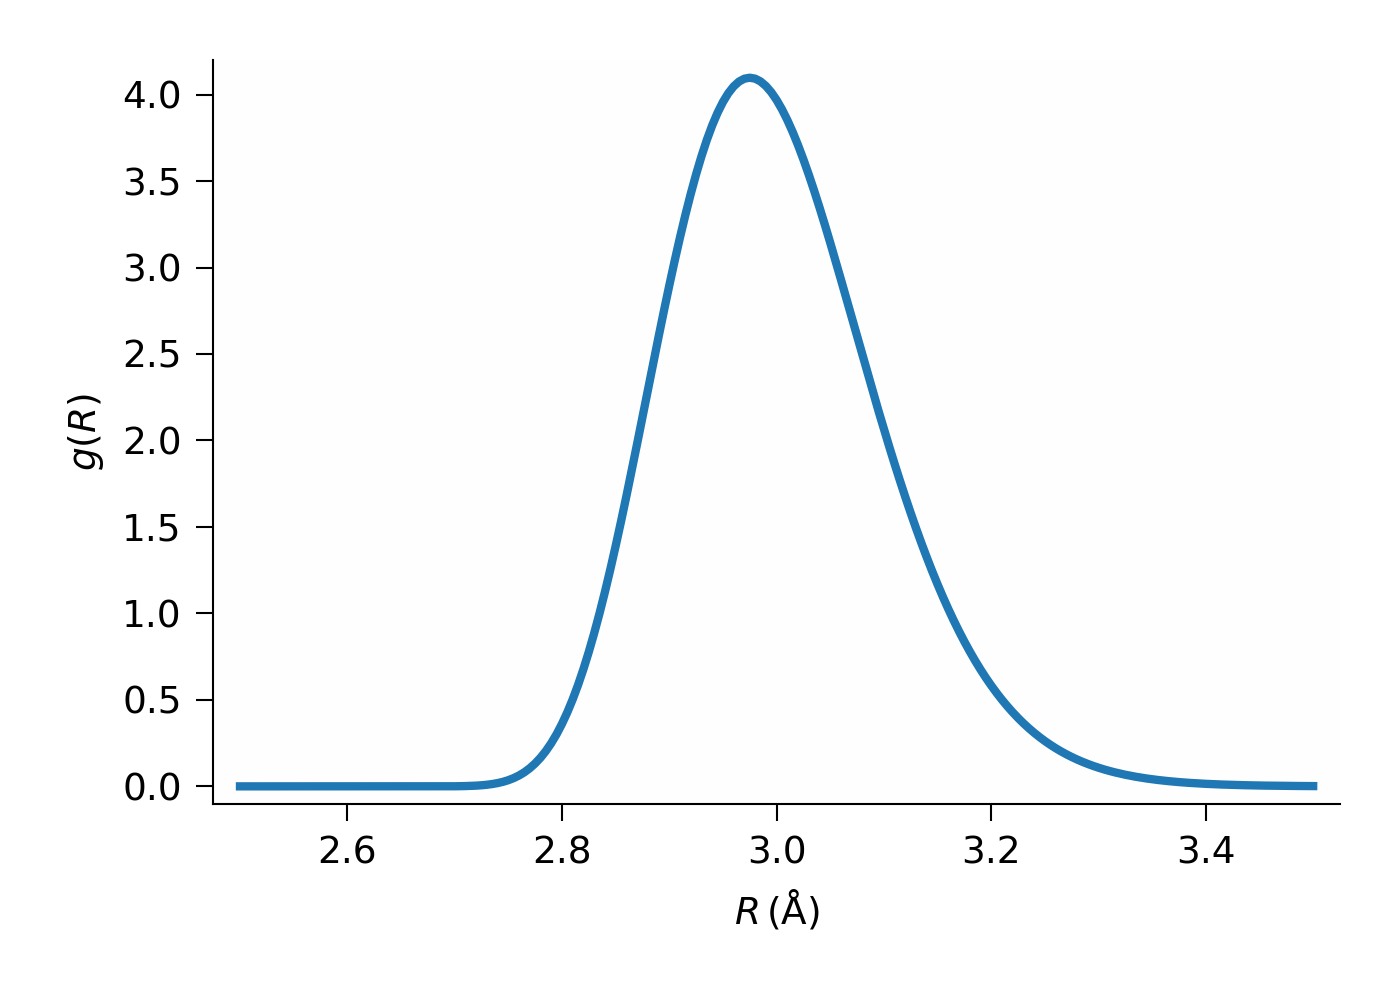
\includegraphics[width=60mm]{figs/errors/gnxas}
    \end{column}
  \end{columns}
\end{cenpage}
\end{slide}


\begin{slide}{EXAFS and The Pair Distribution Function}


  \begin{cenpage}{135mm}
  To fully account for a highly disordered local structure, we should use

\[
    \chi(k)  = \Biggl\langle \sum_j {\frac{f_j(k)e^{i2kR_j + \delta_j(k)}}{kR_j^2}} \Biggr\rangle
\]

where $ \langle x \rangle = \int dR\, x \, g(R) / \int dR\, g(R) $ --
averaging over the billions+ of snapshots.

\vmm\pause
$R$ won't change too much, so we'll neglect the changes to $1/R^2$:

\[
  \chi \approx
  \sum_j {f_j(k){\frac{e^{ i\delta_j(k)} }{kR_j^2}}}   \biggl\langle e^{i2kR_j}  \biggr\rangle
\]

each path in the sum now has a $g(R)$ with respect to the absorbing atom.

\vmm \hrule \vmm \onslide+<3->

The {\RedEmph{the cumulant expansion}} relates $\langle e^x\rangle$ to $\langle x \rangle$, the moments of $g(x)$:


\[ \biggl\langle e^{i2kR} \biggr\rangle
= \exp \bigg[ \sum_{n=1}^{\infty} { \frac{(2ik)^n}{n!}}C_n  \bigg].
\]



\vfill
\end{cenpage}
\end{slide}

%% Slide
\begin{slide}{The Cumulants and Moments of a Distribution Function}

  \begin{cenpage}{135mm}
  The cumulants $C_n$ of $g(R)$ are related to the moments of $g(R)$:
  $\langle r^n \rangle$,

  with $r= R - R_0$ and $R_0$ is the centroid of the distribution:

  \vmm

    \begin{tabular}{lll}
      $C_1 = \Delta R$  & {\BlueEmph{\tt{deltar}}}    & $ = \langle r \rangle    $    \\
      $C_2  = \sigma^2$ &  {\BlueEmph{\tt{sigma2}}} & $ = \langle r^2 \rangle - \langle r \rangle^2    $   \\
      $ C_3 $ & {\BlueEmph{\tt{third}}} & $ = \langle r^3 \rangle - 3 \langle r^2 \rangle
      \langle r \rangle  + 2 \langle r \rangle^3   $    \\
      $ C_4 $ & {\BlueEmph{\tt{fourth}}} & $ =  \langle r^4 \rangle - 3 \langle r^2 \rangle^2
      - 4\langle r^3 \rangle \langle r \rangle
      +12  \langle r^2 \rangle  \langle r \rangle^2
      - 6\langle r \rangle^4  $   \\
    \end{tabular}

    \vmm

    \begin{postitbox}{80mm}
    $C_3$ (the {\RedEmph{third cumulant}}) can be important in many cases.
  \end{postitbox}

    \vmm\hrule\vmm
    \onslide+<2->

\begin{columns}
  \begin{column}{70mm}

    But: Sometimes, the cumulant expansion isn't good enough.  One can also build models by using
    paths spaced in $R$ (say, at 0.2 {\AA} steps), and model the amplitude of each Path with a
    distribution like (following GNXAS):

    \[    g(R, N, R_0, \sigma, \beta) = \frac{2N [  e^{-\alpha} \alpha^{q-1}]}{\sigma\beta\Gamma(q) }\]

    where  $\alpha = q + 2(R-R_0)/(\beta\sigma)$,  and $q = 4/\beta^2$

\vspace{5mm}

    \end{column}
  \begin{column}{65mm}
    \onslide+<2->
      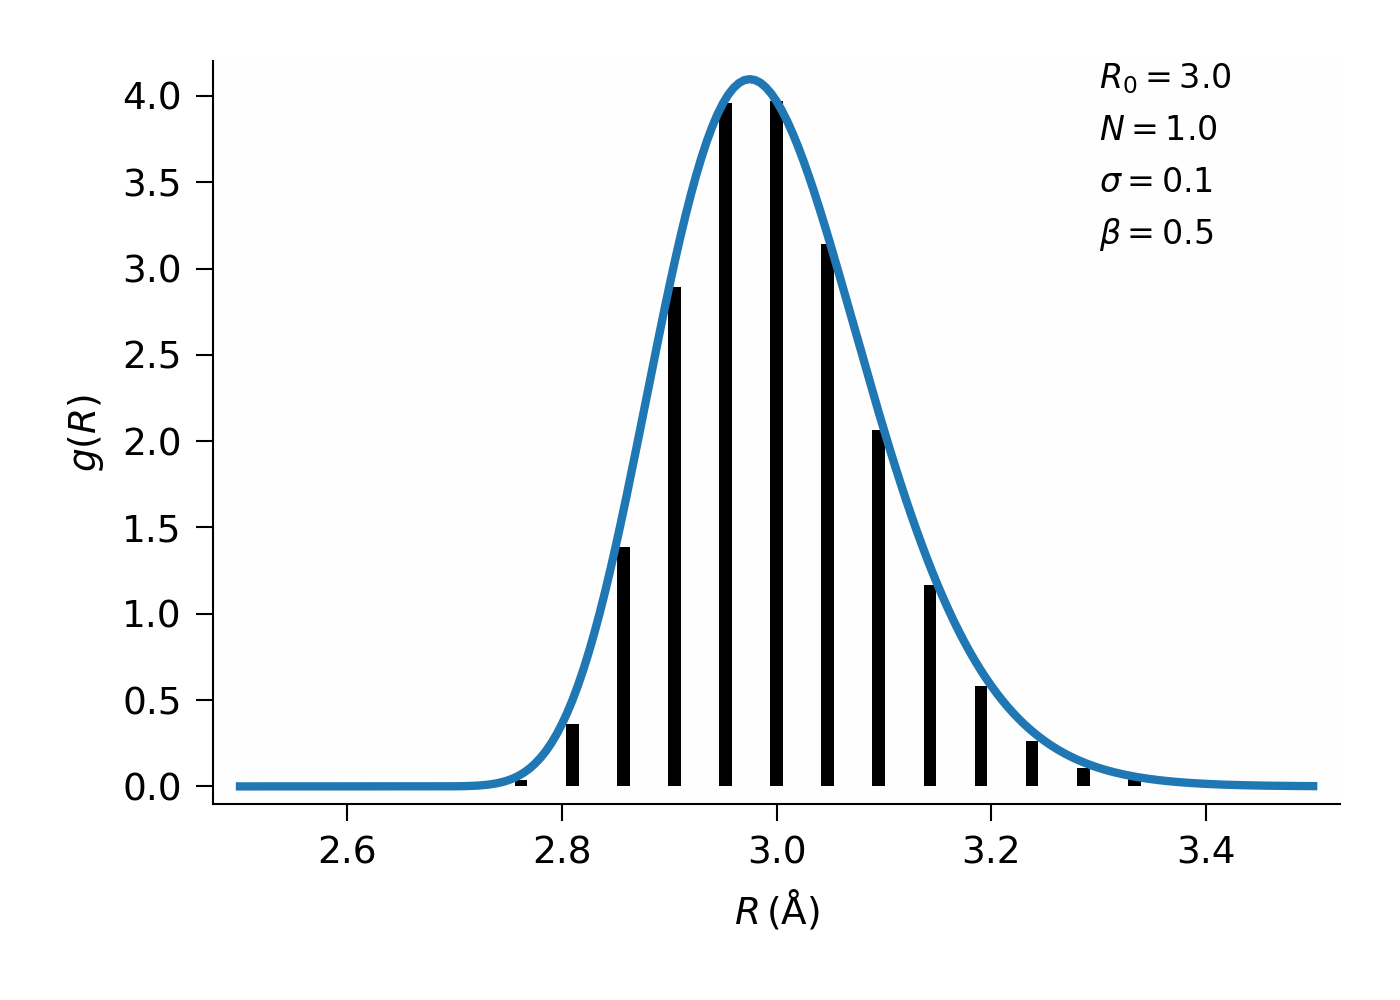
\includegraphics[width=60mm]{figs/errors/gnxas_histogram}
    \end{column}
  \end{columns}

  \end{cenpage}
\end{slide}
